\subsection{Bewertung der Energiebezogenen Leistung}
\subsubsection{Definition von Energieleistungskennzahlen}
Im Rahmen der Planungsphase des PDCA-Zyklus verpflichtet die DIN EN ISO 50001:2018-12 Organisationen zur Festlegung von Energieleistungskennzahlen 
(\cite[S. 7]{DIN50001.2018}).
Eine Energieleistungskennzahl, auch EnPi (en: energy performance indicator) gennant, ist ein Maß oder eine Einheit der energiebezogenen Leistung, wie Sie von der Organisation festgelegt ist 
(\cite[Kapitel 3.4.4]{DIN50001.2018}), und ist somit ein Maßstab für den Vergleich der energiebezogenen Leistung (\cite[Kapitel A.6.4]{DIN50001.2018}). 
Eine Energieleistungskennzahl wird durch einen EnPI-Wert zu einem bestimmten Zeitpunkt oder über einen bestimmten Zeitraum quantifiziert (\cite[Kapitel 3.4.5]{DIN50001.2018}).
EnPI Werte finden Verwendung in der gesamten Organisation und in verschiedenen Teilen der Organisation (\cite[S. 13]{DIN50006.2024}). 
EnPIs ermöglichen einen Vergleich zwischen unterschiedlichen Untersuchungsgegenständen, können zeitliche Veränderungen der energiebezogenen Leistung darstellen und dienen als 
Zielvorgaben und zur Erfolgskontrolle (\cite[S. 2]{Hohnhold.2013}).
Sie bilden nach Hohnhold (2013, S. 2) den Mittelpunkt jeder Bewertung von Energieeffizienz und verdichten Informationen über den Energieverbrauch und dessen Struktur in einer 
Organisation. 
Folglich bilden EnPIs und EnPI-Werte die Grundlage der energiebezogenen Leistung und deren Verbesserung, und sind somit eine Eingangsgröße für die Managementbewertung der energiebezogenen Leistung 
in der Prüfungsphase des PDCA-Zyklus (\cite[Kapitel 9.3.3]{DIN50001.2018}).

Energieleistungskennzahlen hängen mit energetischen Ausgangsbasen zusammen und können Organisationen in die Lage versetzen eine Verbesserung der energiebezogenen Leistung, anhand von verbesserungen bei EnPI-Werten 
im zeitlichen Verlauf im Verhältnis zur entsprechenden energetischen Ausgangsbasis, nachzuweisen (\cite[Kapitel 0.3]{DIN50001.2018}).
Eine Energetische Ausgangsbasis, auch EnB (en: energy baseline) ist von der DIN EN ISO 50001:2018-12 definiert als quantifizierbarer(e) Referenzpunkt(e) für einen Vergleich der energiebezogenen 
Leistung und beruht auf Daten aus einem festgelegten Zeitabschnitt und/oder auf Bedingungen wie von der Organisation festgelegt(\cite[Kapitel 3.4.7]{DIN50001.2018}). 

\begin{figure}[H]
    \centering
    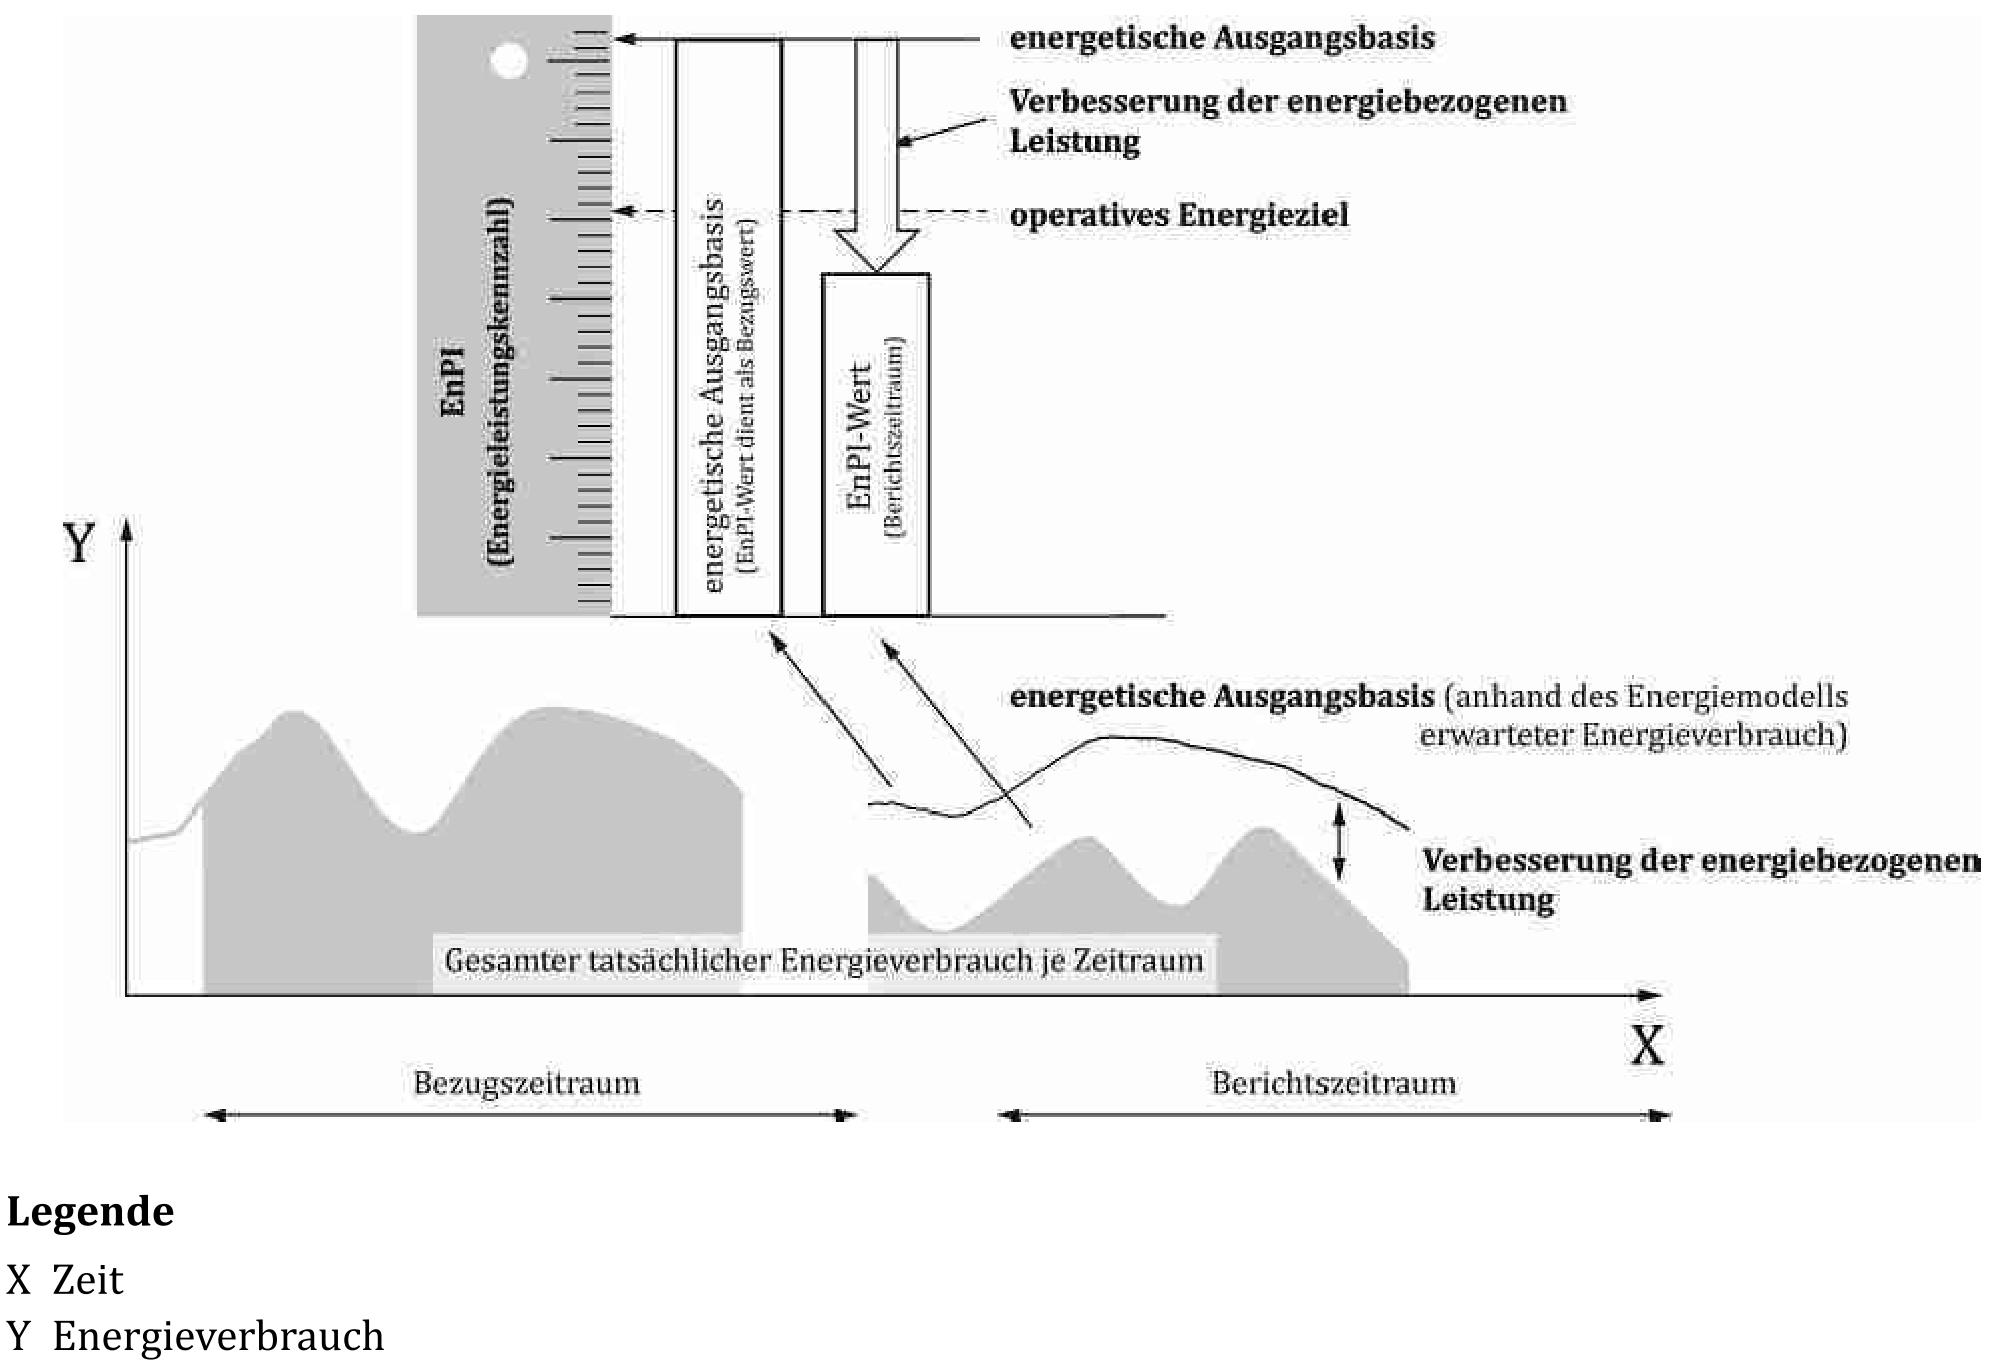
\includegraphics[width=1\textwidth]{../../Ressourcen/Abbildungen/ISO_50006_Beispiel_EnPI_EnB.jpg}
    \caption{Beispiel für die konzeptuelle Beziehung zwischen der energiebezogenen Leistung, EnPIs, EnBs, EnPI-Werten und operativen Energiezielen. (Darstellung der E DIN ISO 50006:2024-07 (2024, S. 14))}
    \label{fig:Beziehung_EnPI_EnB_ISO_50006}
\end{figure}

Die E DIN ISO 50006:2024-07 zeigt ein Beispiel für die Beziehungen zwischen der energiebezogenen Leistung, EnPIs, EnBs, EnPI-Werten und operativen Energiezielen 
in Abbildung \eqref{fig:Beziehung_EnPI_EnB_ISO_50006} auf.
Hier wird der Energieverbrauch über einen Bezugszeitraum als Energieleistungskennzahl definiert.
Die energetische Ausgangsbasis stellt anhand des Energiemodells den erwarteten Energieverbrauch.
Das operative Energieziel gibt den Zielwert des EnPI-Werts im Bezugszeitraum an. 
Die differenz zwischen dem EnB und der EnPI ergibt die Verbesserung der Energiebezogenen Leistung.
Neben der Auskunft über die relevanten Bestandteile zum Nachweis der energiebezogenen Leistung, gibt das Beispiel (vgl. Abbildung \eqref{fig:Beziehung_EnPI_EnB_ISO_50006}) 
zwei Perspektiven auf die Auswertung der genannten Komponenten.
So wird in der unteren Visualisierung die Verbesserung der energiebezogenen Leistung über einen Bezugszeitraum in einem Zeit-Energieverbrauch-Graphen dargestellt.
Diese Art der Visualisierung ermöglicht Erkenntnisgewinne bezüglich des Zeitabhängigen Verhaltens des EnPI-Werts und kann unter anderem zur Identifkation des 
einflusses zeitabhängiger relevanter Variablen wie saisonaler Wetterbedingungen genutzt werden. 
Die Obere Visualisierung aggregiert die EnPI-Werte und die EnB über den Bezugszeitraum zu einzelnen Werten. 
Anhand dieser Werte kann die Erfüllung oder nicht-Erfüllung des operativen Energieziels im Bezugszeitraum evaluiert werden.

\subsubsection{Arten von Kennzahlen aus statistisch-methodischer Perspektive}

\begin{figure}[H]
    \centering
    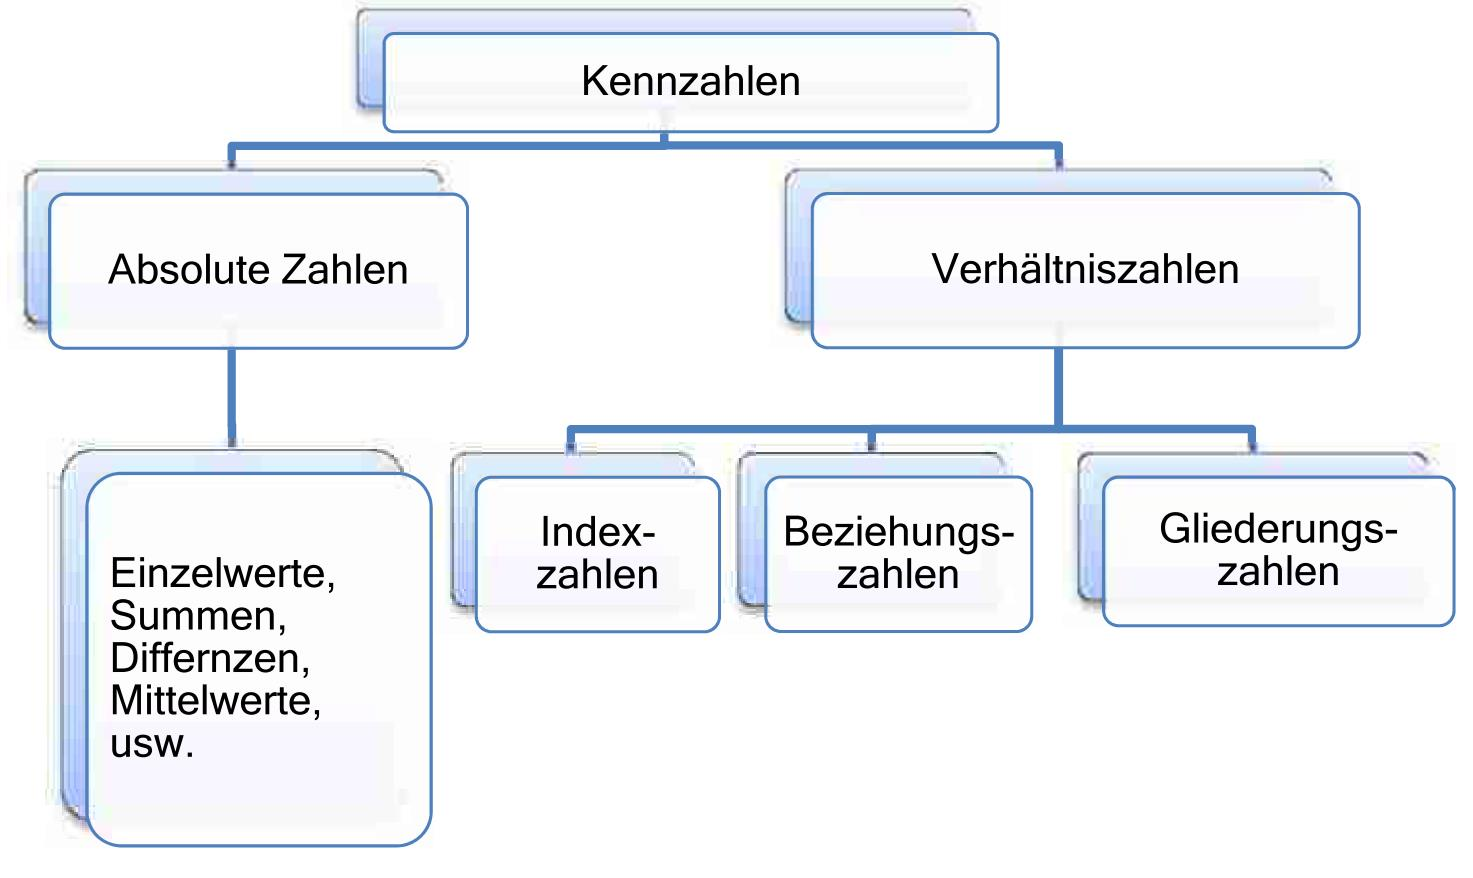
\includegraphics[width=1\textwidth]{../../Ressourcen/Abbildungen/Arten_Kennzahlen_Hohnhold.jpg}
    \caption{Arten von Kennzahlen. (Darstellung von Hohnhold (2013, S. 4))}
    \label{fig:Arten_Kennzahlen}
\end{figure}

Grundsätzlich lassen sich Kennzahlen aus statistisch-methodischer Sicht in zweit Klassen unterteilen: absolute Zahlen und Verhältniszahlen (vgl. Abbildung \eqref{fig:Arten_Kennzahlen}).
Absolute Zahlen werden durch Einzelwerte, Summen, Differenzen oder Mittelwerten abgebildet und eignen sich aufgrund der absoluten Betrachtung auf Aufwandsseite nicht zur Bewertung der Energieeffizienz (\cite[S. 2]{Hohnhold.2013}).
So fällt auch der in Abbildung \eqref{fig:Beziehung_EnPI_EnB_ISO_50006} dargestellte Energieverbrauch in einem Bezugszeitraum in die Klassifizierung einer absoluten Kennzahl (\cite[S. 2]{Hohnhold.2013}).
Obwohl absolute Zahlen nicht zur Bewertung der Energieeffizienz geeignet sind, können sie wie in Abbildung \eqref{fig:Beziehung_EnPI_EnB_ISO_50006} visualisert 
auskunft über die Verbesserung der energiebezogenen Leistung geben.
Verhältniszahlen bilden einen Quotienten aus zusammenhängenden Größen und sind dadurch besser zur Analyse der Energieeffizienz geeignet (\cite[S. 3]{Hohnhold.2013}).
Die Auswahl der Bezugsgrößen zur Bildung der Verhältniszahlen hängt von der untersuchten Organisation und der untersuchten Branche ab (\cite[S. 3]{Hohnhold.2013}). 
Im erarbeiteten Bilanzraumkonzept für Organisationen im tertiären Wirtschaftssektor (vgl. Abbildung \eqref{fig:Übersicht_Bilanzräume}) können die auf der aufwandsseitig erfassten Ressourcen ins 
Verhältnis zu der jeweiligen Nutzengrößen gesetzt werden.

\subsubsection{Grenzen von Energieleistungskennzahlen}
Um die Vergleichbarkeit von Energiekennzahlen zu gewährleisten müssen die Bilanzräume von Anlagen, Prozessen und Bereichen bekannt sein (\cite[S. 310]{Engelmann.2015}).
Der Bilanzraum beeinflusst eine Energiekennzahl durch seine räumliche und zeitliche Abgrenzung (\cite[S. 6]{Hohnhold.2013}).
Die E DIN ISO 50006:2024-07 formuliert konkrete Anforderungen die bei der Festlegung von Grenzen eines EnPI zu beachten sind.
So müssen bei der Definition einer EnPI-Grenze nach E DIN ISO 50006:2024-07 folgende Aspekte berücksichtigt werden.

\begin{itemize}
    \item Die organisatorische Verantwortlichkeiten im Bezug auf das Energiemanagement, einschließlich des Umfangs, in dem die 
    Organisation Einfluss auf ihre energiebezogene Leistung hat beziehungsweise diese steuern kann (\cite[Kapitel 5.3]{DIN50006.2024}). 
    \item Die wesentlichen Energieeinsätze (\cite[Kapitel 5.3]{DIN50006.2024}). 
    \item Einrichtungen, Ausrüstungen, Systeme oder energieverbrauchende Prozesse die die Organisation zu isolieren sowie zu steuern wünscht (\cite[Kapitel 5.3]{DIN50006.2024}). 
    \item Die Einfachheit der Eingrenzung der EnPI-Grenze durch die Messung von Energieverbrauch und relevanten Variablen (\cite[Kapitel 5.3]{DIN50006.2024}). 
    \item Die Grenze des Energiemanagementsystems (\cite[Kapitel 5.3]{DIN50006.2024}). 
    \item Die verfügbaren Daten zum Energievebrauch und zu relevanten Vairablen (\cite[Kapitel 5.3]{DIN50006.2024}). 
\end{itemize}

Daraus ergeben sich die drei primären Grenzniveaus: einzeln, systembezogen und organisatorisch (vgl. Abbildung ) (\cite[Kapitel 5.3]{DIN50006.2024}). 
\begin{figure}[H]
    \centering
    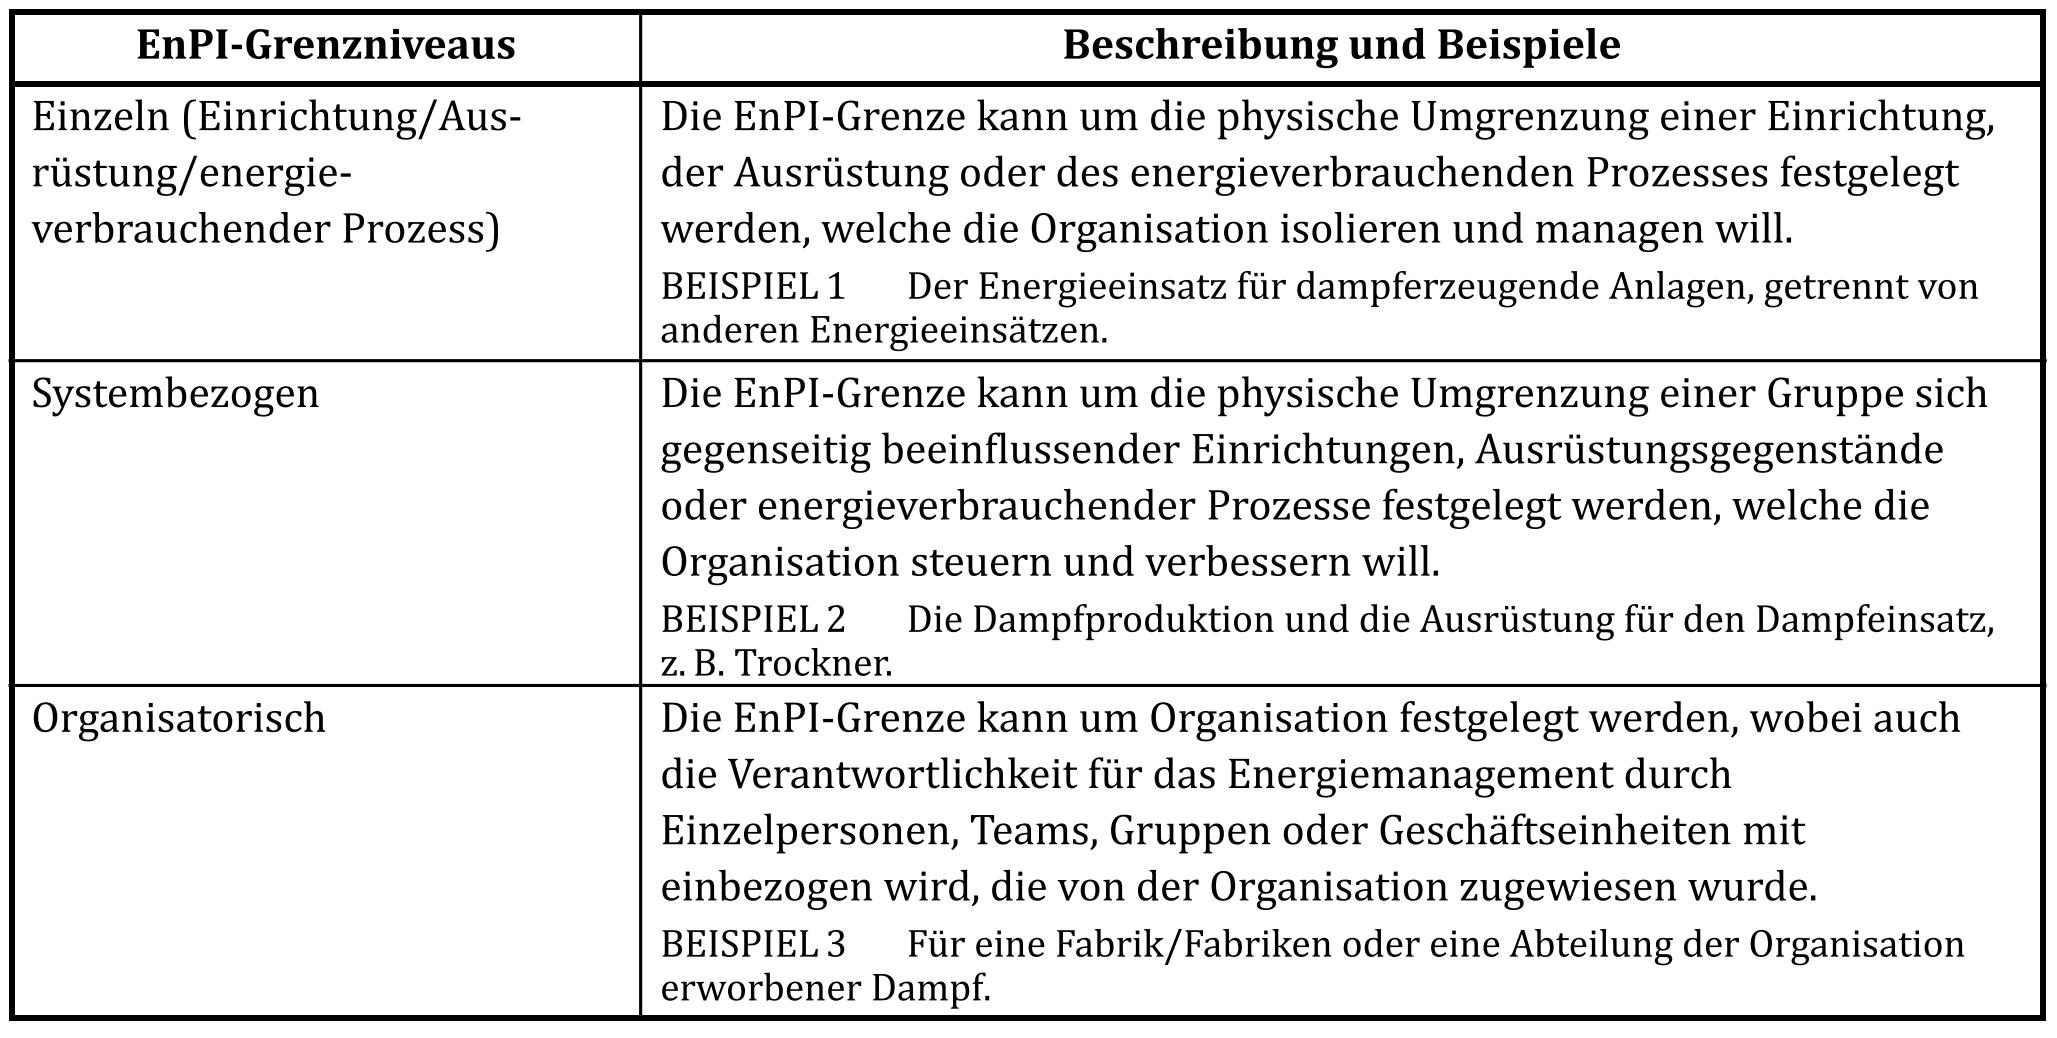
\includegraphics[width=1\textwidth]{../../Ressourcen/Abbildungen/EnPI_Grenzniveaus_ISO_50006.jpg}
    \caption{Die drei EnPI-Grenzniveaus. (Darstellung der E DIN ISO 50006:2024-07 (2024, S. 16))}
    \label{fig:EnPI_Grenzniveaus}
\end{figure}
In Organisationen die keine materiellen Güter Produzieren, also alle Organisationen des tertiären Wirtschaftssektors, eignen sich Gebäude am besten zur 
Abgrenzung der EnPIs (\cite[S. 9]{Fichera.2020}). 
Im rahmen der Bestimmtung der EnPI-Grenzen sollen Organisationen nach E DIN ISO 50006:2024-07 (2024, S. 17) die für die einzelnen Grenzen relevanten Variablen 
bestimmen.
Außerdem ist es für die statistische Analyse der EnPI-Werte notwendig dass der Energieverbrauch und die Daten der zugehörigen relevanten Variablen 
die gleichen Zeitintervalle umfassen (\cite[S. 20]{DIN50006.2024}).
Folglich ist auch eine Zeitliche Abgrenzung der EnPIs notwendig.

\subsubsection{Datengetriebene Auswertung von Energieleistungskennzahlen}